\section{Experimental Setup and Measurements}
\label{sec:procedure}
\subsection{The Laser}
\label{sec:lasersetup}
The laser system consists of the diode laser a lens used to collimate the beam, an electric heating system
and the diffraction grating. These components can be seen in Figure~\ref{fig:laserhead}.
\begin{figure}[H]
  \centering
  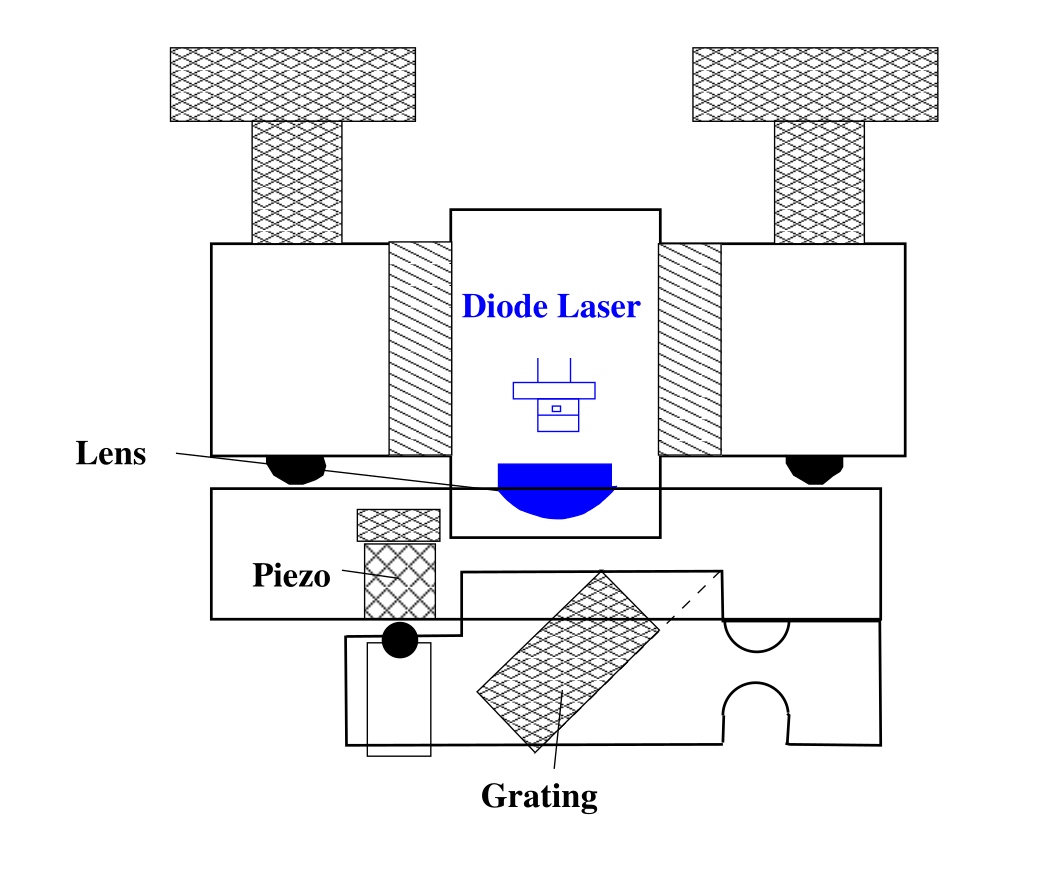
\includegraphics[scale=0.25]{./pictures/Laser-Head.png}
  \caption{Display of the laser assembly~\cite{V61}.}
  \label{fig:laserhead}
\end{figure}
\noindent
The diode laser uses a p-n semiconductor made from aluminium gallium arsenide (AlGaAs), with facets on both ends
of the chip with $\SI{100}{\percent}$ and $\SI{15}{\percent}$ reflectivity respectively. The external cavity
is realised through the diffraction grating in Littrow configuration.
To adjust the laser, using an indication card, a photodiode or a CCD camera is required because the laser
wavelength is in the near infrared region of the spectrum and can therefore not be seen by the human eye.
To adjust the external cavity, the angular orientation of the optical grating is modified until the first and
second order diffraction overlap on the monitor of the CCD camera. If this is the case, the second order of
diffraction is routed back into the laser diode. The maximise the output power, the CCD camera is replaced by a
photodiode and a connected voltmeter. Then, the lens is adjusted until the maximum power is reached.
\subsection{Measurements}
\label{sec:measurements}
\subsubsection{The lasing Threshold and Characteristics}
\label{sec:threshold}
To study the characteristics of the diode laser, the current threshold for the lasing process is measured.
For this, a piece of paper is placed in the laser beam in front of the laser. The light reflected by the paper
is observed with the CCD camera. The injection current is increased; at the threshold, the brightness of the
reflected beam suddenly increases and a speckle pattern is visible. Mode hopping is observed and documented
using an oscilloscope. Additionally, the external cavity length is varied and the resulting effect measured.
\subsubsection{The Hyperfine Splitting of Rubidium}
\label{sec:rubidium}
For the measurement of the hyperfine splitting of rubidium, a cell containing $\SI{72}{\percent} \ ^{85}\text{Rb}$
and $\SI{28}{\percent} \ ^{87}\text{Rb}$, a heating device, a cooling finger as well as a pair of Helmholtz coils
is placed in the laser beam. The Helmholtz coils have a radius of $r=\SI{87.4}{\milli\meter}$ and $320$ turns.
They are made of copper. Here, two photodiodes are used to suppress noise. The full structure can be seen
schematically in Figure~\ref{fig:structure}.
\begin{figure}[H]
  \centering
  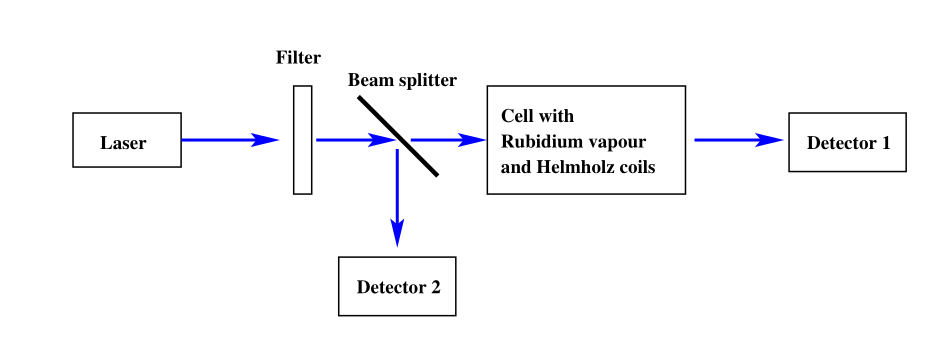
\includegraphics[scale=0.38]{./pictures/structure.png}
  \caption{The experimental setup for measuring the hyperfine splitting of rubidium~\cite{V61}.}
  \label{fig:structure}
\end{figure}
\noindent
To measure the hyperfine splitting, the transmitted light is measured as a function of the laser frequency.
